\documentclass[tikz,border=12pt]{standalone}
\usepackage{amsmath}
\usepackage{amssymb}
\usepackage{tikz}
\usetikzlibrary{calc,arrows.meta,decorations.pathmorphing,decorations.pathreplacing,positioning}

\begin{document}
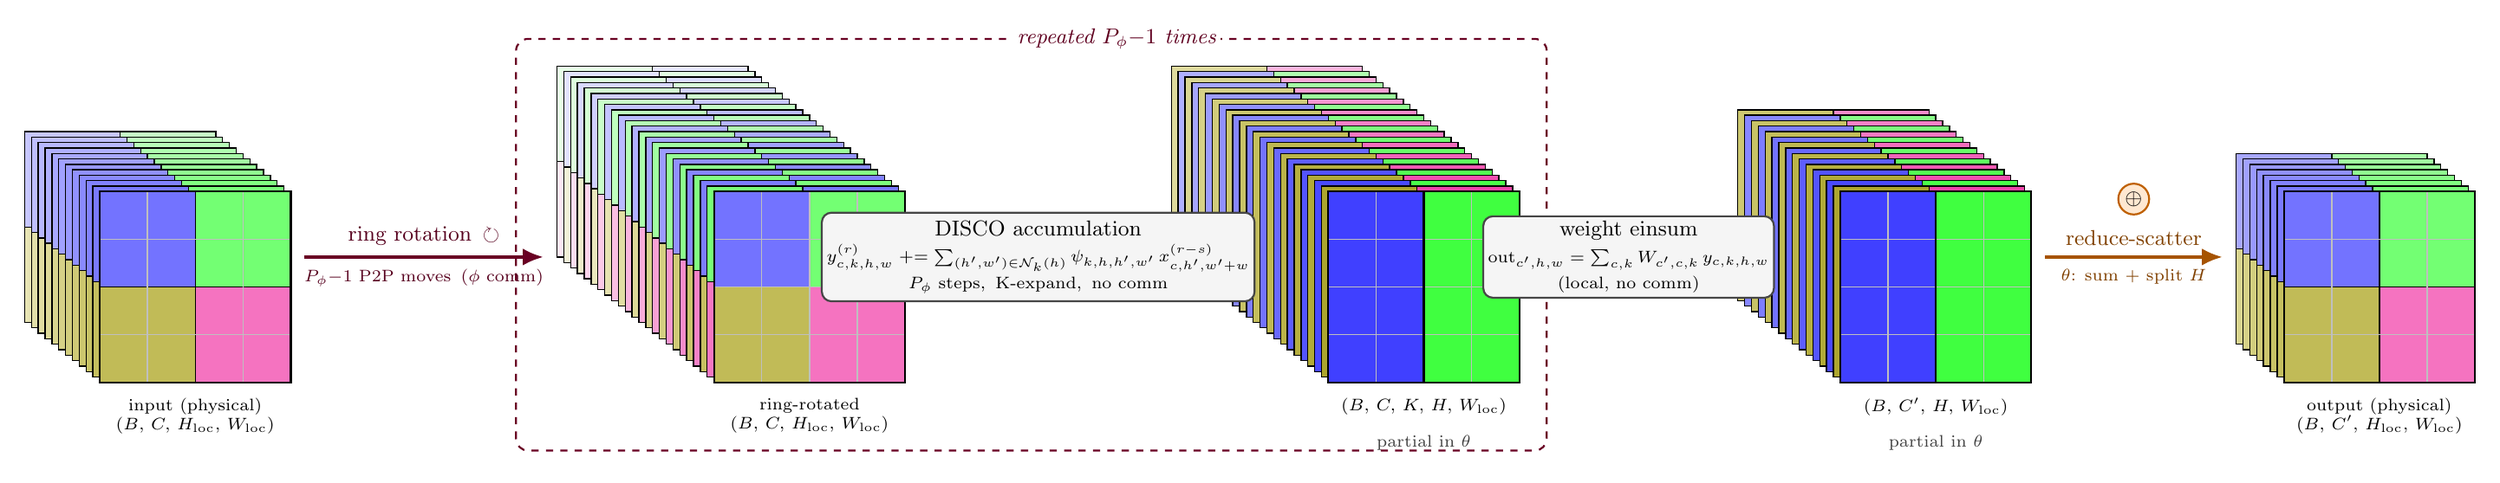
\begin{tikzpicture}[
  font=\sffamily,
  >=Latex,
  line width=0.5pt,
]

% ============================================================================
% Distributed DISCO conv — RING variant, reduce-scatter on the polar H dim
%
% Code path (_distributed_disco_fwd_ring + _RingDiscoConvS2Fn):
%   (B, C, H_loc, W_loc)                input — physical, H×W sharded
%   ── ring loop  (P_phi P2P rotations, DISCO contraction each step) ──>
%                                       (B, C, K, H_out, W_loc)
%                                       full H_out per rank (partial in θ),
%                                       channels stay LOCAL throughout.
%   ── local weight einsum (no comm) ──>
%                                       (B, C', H_out, W_loc)
%                                       K collapsed, channels projected C → C'
%   ── reduce-scatter polar on H ──>    (B, C', H_loc, W_loc)   output
%
% Total comm: P_phi-1 ring P2Ps on the azimuth comm + 1 reduce-scatter on
% the polar comm. ZERO all-to-alls (vs. 2 in the A2A variant) and channels
% never move across ranks — only W chunks rotate.
% ============================================================================

% per-card stack offsets
\def\dxIn{-0.10}\def\dyIn{0.08}

% ---------- helper: stacked yxgrid (channels = card stack on 2x2 spatial grid) ----
% args: cx, cy, halfwidth, n-cards, front-saturation, label
\newcommand{\yxstack}[6]{%
  \pgfmathtruncatemacro{\nm}{#4-1}%
  \foreach \k in {0,...,\nm}{%
    \pgfmathtruncatemacro{\j}{\nm-\k}%
    \pgfmathsetmacro{\ox}{#1 + \j*\dxIn}%
    \pgfmathsetmacro{\oy}{#2 + \j*\dyIn}%
    \pgfmathtruncatemacro{\sh}{#5 - \j*3}%
    \fill[blue!\sh!white,draw=black]    ({\ox-#3},{\oy})    rectangle ({\ox},{\oy+#3});%
    \fill[green!\sh!white,draw=black]   ({\ox},{\oy})       rectangle ({\ox+#3},{\oy+#3});%
    \fill[olive!\sh!white,draw=black]   ({\ox-#3},{\oy-#3}) rectangle ({\ox},{\oy});%
    \fill[magenta!\sh!white,draw=black] ({\ox},{\oy-#3})    rectangle ({\ox+#3},{\oy});%
  }%
  \foreach \i in {-1,1}{
    \draw[gray!50] ({#1+\i*#3/2},{#2-#3}) -- ({#1+\i*#3/2},{#2+#3});
    \draw[gray!50] ({#1-#3},{#2+\i*#3/2}) -- ({#1+#3},{#2+\i*#3/2});
  }
  \draw[thick] ({#1-#3},{#2-#3}) rectangle ({#1+#3},{#2+#3});
  \node[anchor=north,font=\scriptsize,align=center] at (#1,{#2-#3-0.10}) {#6};
}

% ---------- helper: ring-rotated stack (mid-ring-loop illustration) ----------
% Shows what happens to the W chunks during the ring loop: each rank
% cycles through the other ranks' W chunks via P2P rotation. We render
% 2*Np cards in Np pairs — within each pair:
%   card 0 (ring step 0): original 2x2 yxgrid coloring — each rank holds
%       its own W chunk (NW=blue, NE=green, SW=olive, SE=magenta).
%   card 1 (ring step 1): LEFT/RIGHT colours SWAPPED — after one rotation
%       each azimuth rank holds its neighbour's W chunk
%       (NW=green, NE=blue, SW=magenta, SE=olive).
% Channels never move, just the W chunks circulate. Shape is unchanged
% from the input.
%
% args: cx, cy, halfwidth, n-pairs, front-saturation, label
\newcommand{\ringpaired}[6]{%
  \pgfmathtruncatemacro{\nTot}{2*#4-1}%
  \foreach \k in {0,...,\nTot}{%
    \pgfmathtruncatemacro{\j}{\nTot-\k}%
    \pgfmathsetmacro{\ox}{#1 + \j*\dxIn}%
    \pgfmathsetmacro{\oy}{#2 + \j*\dyIn}%
    \pgfmathtruncatemacro{\sh}{#5 - \j*2}%
    \pgfmathtruncatemacro{\step}{mod(\j,2)}%   % 0 = original, 1 = W-swapped
    \ifnum\step=0
      \fill[blue!\sh!white,draw=black]    ({\ox-#3},{\oy})    rectangle ({\ox},{\oy+#3});%
      \fill[green!\sh!white,draw=black]   ({\ox},{\oy})       rectangle ({\ox+#3},{\oy+#3});%
      \fill[olive!\sh!white,draw=black]   ({\ox-#3},{\oy-#3}) rectangle ({\ox},{\oy});%
      \fill[magenta!\sh!white,draw=black] ({\ox},{\oy-#3})    rectangle ({\ox+#3},{\oy});%
    \else
      \fill[green!\sh!white,draw=black]   ({\ox-#3},{\oy})    rectangle ({\ox},{\oy+#3});%
      \fill[blue!\sh!white,draw=black]    ({\ox},{\oy})       rectangle ({\ox+#3},{\oy+#3});%
      \fill[magenta!\sh!white,draw=black] ({\ox-#3},{\oy-#3}) rectangle ({\ox},{\oy});%
      \fill[olive!\sh!white,draw=black]   ({\ox},{\oy-#3})    rectangle ({\ox+#3},{\oy});%
    \fi
  }%
  % Full 4x4 gridlines. Vertical centerline THICK (W is still
  % azimuth-split — left vs right cols are a rank boundary); horizontal
  % gray (polar split still intact too — top vs bottom rows ARE a rank
  % boundary, but the swap only happens in W direction, so visually the
  % horizontal line is just a regular gridline here).
  \foreach \i in {-1,1}{
    \draw[gray!50] ({#1+\i*#3/2},{#2-#3}) -- ({#1+\i*#3/2},{#2+#3});
    \draw[gray!50] ({#1-#3},{#2+\i*#3/2}) -- ({#1+#3},{#2+\i*#3/2});
  }
  \draw[gray!50] ({#1-#3},#2) -- ({#1+#3},#2);
  \draw[gray!50] (#1,{#2-#3}) -- (#1,{#2+#3});
  \draw[thick] ({#1-#3},{#2-#3}) rectangle ({#1+#3},{#2+#3});
  \node[anchor=north,font=\scriptsize,align=center] at (#1,{#2-#3-0.10}) {#6};
}

% ---------- helper: column-paired stack (partial-in-θ with W still azimuth-split) ----
% Captures the post-ring (and post-einsum, pre-RS) state in the ring algorithm:
%   * channels stay LOCAL (so the stack runs through all C cards per rank),
%   * each rank holds the FULL H_out (partial values to be summed by RS),
%   * W is still azimuth-split per rank.
% We render Np channel pairs of 2 cards each (=> 2*Np cards). Within a pair:
%   card 0 (polar 0 partial): blue (left cols, azimuth 0) | green (right cols, azimuth 1)
%   card 1 (polar 1 partial): olive (left cols)            | magenta (right cols)
% All Np pairs share the same colour pattern (channels are not split across
% ranks in the ring algorithm). Reduce-scatter will pairwise sum each polar
% pair and split the rows → consolidated Np-card yxstack at B4.
%
% args: cx, cy, halfwidth, n-pairs, front-saturation, label
\newcommand{\colpaired}[6]{%
  \pgfmathtruncatemacro{\nTot}{2*#4-1}%
  \foreach \k in {0,...,\nTot}{%
    \pgfmathtruncatemacro{\j}{\nTot-\k}%
    \pgfmathsetmacro{\ox}{#1 + \j*\dxIn}%
    \pgfmathsetmacro{\oy}{#2 + \j*\dyIn}%
    \pgfmathtruncatemacro{\sh}{#5 - \j*2}%
    \pgfmathtruncatemacro{\pol}{mod(\j,2)}%    % 0 = polar-0 partial, 1 = polar-1
    \ifnum\pol=0
      \fill[blue!\sh!white,draw=black]    ({\ox-#3},{\oy-#3}) rectangle ({\ox},{\oy+#3});%
      \fill[green!\sh!white,draw=black]   ({\ox},{\oy-#3})    rectangle ({\ox+#3},{\oy+#3});%
    \else
      \fill[olive!\sh!white,draw=black]   ({\ox-#3},{\oy-#3}) rectangle ({\ox},{\oy+#3});%
      \fill[magenta!\sh!white,draw=black] ({\ox},{\oy-#3})    rectangle ({\ox+#3},{\oy+#3});%
    \fi
  }%
  % Full 4x4 gridlines. Horizontal centerline is GRAY (each rank holds the
  % full H — no rank boundary on rows); vertical centerline is THICK (W is
  % still azimuth-split — left cols vs right cols ARE a rank boundary).
  \foreach \i in {-1,1}{
    \draw[gray!50] ({#1+\i*#3/2},{#2-#3}) -- ({#1+\i*#3/2},{#2+#3});
    \draw[gray!50] ({#1-#3},{#2+\i*#3/2}) -- ({#1+#3},{#2+\i*#3/2});
  }
  \draw[gray!50] ({#1-#3},#2) -- ({#1+#3},#2);
  \draw[thick] (#1,{#2-#3}) -- (#1,{#2+#3});
  \draw[thick] ({#1-#3},{#2-#3}) rectangle ({#1+#3},{#2+#3});
  \node[anchor=north,font=\scriptsize,align=center] at (#1,{#2-#3-0.10}) {#6};
}

% ============================================================================
% LAYOUT — four square blocks. Channels stay LOCAL across ranks throughout
% the ring algorithm (no a2as), so the visual story is just three changes
% along the pipeline:
%   1. K-expansion + partial-in-θ after the ring loop  (B1 → B2, sat bump),
%   2. C → C' projection at the local weight einsum     (B2 → B3, channel
%      stack thins from Np_in pairs to Np_out pairs),
%   3. Reduce-scatter folds the polar partials and splits the rows
%      (B3 → B4, paired stack collapses to a normal yxstack).
% ============================================================================
\def\halfw{1.4}
\pgfmathsetmacro{\cY}{(11*\dyIn)/2}    % arrow baseline = visual mid of a 12-card stack

\def\Nin{12}                            % input C channel cards
\def\Nout{8}                            % output C' channel cards (post-einsum)

\def\satPhys{55}                        % physical regime
\def\satK{75}                           % partial-in-θ / K-expanded regime

% --------- B1: physical input (H×W sharded, C local) ---------
\yxstack{0}{0}{\halfw}{\Nin}{\satPhys}{input (physical)\\$(B,\,C,\,H_\text{loc},\,W_\text{loc})$};

% --------- B2: ring-rotation illustration — W chunks circulate, shape unchanged ----
% 2*\Nin = 24 cards in \Nin channel pairs. Within each pair: card 0 is
% the original W positions, card 1 is W-swapped (each azimuth rank holds
% its neighbour's W chunk). This visualises the P2P circulation done
% during the ring loop; the data shape is identical to B1.
\def\xR{9.0}
\ringpaired{\xR}{0}{\halfw}{\Nin}{\satPhys}{ring-rotated\\$(B,\,C,\,H_\text{loc},\,W_\text{loc})$};

% --------- B3: post-ring-loop — K-expanded, partial in θ, W still local ---------
% \Nin channel pairs of 2 (= 2*\Nin = 24 cards). Each pair carries the
% polar-0 and polar-1 partial contributions for one channel. RS later
% folds each pair into one card.
\def\xB{18.0}
\colpaired{\xB}{0}{\halfw}{\Nin}{\satK}{$(B,\,C,\,K,\,H,\,W_\text{loc})$};
\node[font=\scriptsize,anchor=north,gray!50!black,align=center]
  at (\xB,{-\halfw-0.65}) {partial in $\theta$};

% --------- B4: post-weight-einsum — K collapsed, C → C', still partial in θ ---------
% Same column-paired pattern as B3 but the channel pair count drops from
% \Nin → \Nout (mirroring the channel projection of the local einsum).
\def\xC{25.5}
\colpaired{\xC}{0}{\halfw}{\Nout}{\satK}{$(B,\,C',\,H,\,W_\text{loc})$};
\node[font=\scriptsize,anchor=north,gray!50!black,align=center]
  at (\xC,{-\halfw-0.65}) {partial in $\theta$};

% --------- B5: output physical (after reduce-scatter on H) ---------
% Pairs collapse to single cards, H goes from full (partial) → H_loc
% (proper, polar-split). Back to standard 2x2 quadrants.
\def\xF{32.0}
\yxstack{\xF}{0}{\halfw}{\Nout}{\satPhys}{output (physical)\\$(B,\,C',\,H_\text{loc},\,W_\text{loc})$};

% --------- iteration box: visually group B2 and B3 as the ring-loop body ----
% Only B2 (post-rotation) and B3 (post-DISCO-accumulation) live inside
% the loop; the weight einsum (A3) and reduce-scatter (A4) downstream
% run once.
\draw[draw=purple!55!black,thick,dashed,rounded corners=5pt]
  (4.7,-2.4) rectangle ({\xB+\halfw+0.4},{\halfw+(2*\Nin-1)*\dyIn+0.4});
\node[font=\small\itshape,purple!50!black,fill=white,inner sep=2pt]
  at ({(\xR+\xB)/2},{\halfw+(2*\Nin-1)*\dyIn+0.4})
  {repeated $P_\phi {-} 1$ times};

% ============================================================================
% ARROWS + LABELS
% B1 / B4 are N-card yxstacks; B2 / B3 are 2N-card colpaired stacks.
% Back-card left edge offset = halfw + (n_cards - 1)*|dxIn| + small pad.
% ============================================================================
\def\xPad{0.20}
\pgfmathsetmacro{\xRightOff}{\halfw+\xPad}                          % +1.6
\pgfmathsetmacro{\xLeftIn}{\halfw+(\Nin-1)*0.10+\xPad}              % -2.7 (Nin=12 yxstack)
\pgfmathsetmacro{\xLeftOut}{\halfw+(\Nout-1)*0.10+\xPad}            % -2.3 (Nout=8 yxstack)
\pgfmathsetmacro{\xLeftPairIn}{\halfw+(2*\Nin-1)*0.10+\xPad}        % -3.9 (Nin=12 colpaired)
\pgfmathsetmacro{\xLeftPairOut}{\halfw+(2*\Nout-1)*0.10+\xPad}      % -3.1 (Nout=8 colpaired)

% --- A1: B1 → B2 (P2P rotations — ring move only, no DISCO yet) ---
\coordinate (a1s) at ({0+\xRightOff},\cY);
\coordinate (a1e) at ({\xR-\xLeftPairIn},\cY);
\draw[-{Latex[length=3mm,width=2.5mm]},very thick,purple!55!black] (a1s) -- (a1e);
\node[font=\small,anchor=south,purple!45!black]
  at ($(a1s)!0.5!(a1e)+(0,0.05)$) {ring rotation\, $\circlearrowright$};
\node[font=\scriptsize,anchor=north,purple!45!black,align=center]
  at ($(a1s)!0.5!(a1e)+(0,-0.05)$) {$P_\phi{-}1$ P2P moves \,($\phi$ comm)};

% --- A2: B2 → B3 (DISCO contraction accumulated over the P_φ ring steps) ---
\coordinate (a2s) at ({\xR+\xRightOff},\cY);
\coordinate (a2e) at ({\xB-\xLeftPairIn},\cY);
\draw[-{Latex[length=3mm,width=2.5mm]},very thick,gray!55!black] (a2s) -- (a2e);
\node[draw=gray!55!black,thick,fill=gray!8,rounded corners,
      minimum width=42mm,minimum height=13mm,align=center,font=\small,inner sep=2pt]
  (disco) at ($(a2s)!0.5!(a2e)$)
  {DISCO accumulation\\
   {\scriptsize $y^{(r)}_{c,k,h,w} \mathrel{+}= \sum_{(h',w')\in\mathcal{N}_k(h)} \psi_{k,h,h',w'}\,x^{(r-s)}_{c,h',w'+w}$}\\
   {\scriptsize $P_\phi$ steps,\, K-expand,\, no comm}};

% --- A3: B3 → B4 (local weight einsum, K collapsed, C → C') ---
\coordinate (a3s) at ({\xB+\xRightOff},\cY);
\coordinate (a3e) at ({\xC-\xLeftPairOut},\cY);
\draw[-{Latex[length=3mm,width=2.5mm]},very thick,gray!55!black] (a3s) -- (a3e);
\node[draw=gray!55!black,thick,fill=gray!8,rounded corners,
      minimum width=36mm,minimum height=11mm,align=center,font=\small,inner sep=2pt]
  (mix) at ($(a3s)!0.5!(a3e)$)
  {weight einsum\\
   {\scriptsize $\mathrm{out}_{c',h,w}=\sum_{c,k} W_{c',c,k}\,y_{c,k,h,w}$}\\
   {\scriptsize (local, no comm)}};

% --- A4: B4 → B5 (reduce-scatter on polar H) ---
\coordinate (a4s) at ({\xC+\xRightOff},\cY);
\coordinate (a4e) at ({\xF-\xLeftOut},\cY);
\draw[-{Latex[length=3mm,width=2.5mm]},very thick,orange!65!black] (a4s) -- (a4e);
\node[font=\small,anchor=south,orange!50!black]
  at ($(a4s)!0.5!(a4e)+(0,0.05)$) {reduce-scatter};
\node[font=\scriptsize,anchor=north,orange!50!black,align=center]
  at ($(a4s)!0.5!(a4e)+(0,-0.05)$) {$\theta$: sum + split $H$};
\node[draw=orange!75!black,thick,fill=orange!18,circle,inner sep=1.2pt,font=\small] (rs)
  at ($(a4s)!0.5!(a4e)+(0,0.85)$) {$\oplus$};

% ============================================================================
% Title (commented — uncomment for a header)
% ============================================================================
%\node[font=\large\bfseries,anchor=south,gray!25!black]
%  at ({(\xB+\xC)/2}, 3.4)
%  {Distributed DISCO conv (ring)};
%
%\node[font=\scriptsize,anchor=south,align=center,gray!45!black,text width=13cm]
%  at ({(\xB+\xC)/2}, 3.0)
%  {\textit{Channels stay local; only W chunks rotate.\,\, P_$\phi$-1 P2Ps + 1 reduce-scatter; no a2as.}};

\end{tikzpicture}
\end{document}
